%! TEX program = lualatex
%        File: main.tex
%     Created: Mar Apr 18 06:00 pm 2017 C
% Last Change: Mar Apr 18 06:00 pm 2017 C
%
\documentclass[11pt, a4paper]{book}
	%\usepackage{pdfsync}
	%\synctex1
	%\usepackage[binding=5mm]{layaureo}
	%\usepackage[showframe]{geometry}
	\pagestyle{plain}
	%\usepackage{syntonly}
	%\syntaxonly
	\usepackage[hidelinks]{hyperref}
	\usepackage{graphicx}
	\usepackage{subfigure}
	\usepackage{xcolor}
	\usepackage{amsmath, amssymb}
		\renewcommand{\epsilon}{\varepsilon}
		\renewcommand{\theta}{\vartheta}
		\renewcommand{\rho}{\varrho}
		\renewcommand{\phi}{\varphi}
	%%%%%%%%%%%%%%%%%%%%%%%%%%%%%%%%%%%%%%%%%
	\usepackage[UKenglish]{babel}
	\usepackage[utf8]{inputenc}
	\usepackage[T1]{fontenc}
	%\usepackage{lmodern}
	\usepackage[lining]{libertine}
	\usepackage[cmbraces, libertine, varg, smallerops]{newtxmath}
	\usepackage{bm}
	\renewcommand{\mathbf}{\bm}
	\usepackage{ebgaramond}
	\usepackage{microtype}
	\usepackage{titlesec}
		\titleformat*{\section}{\Large\swshape}
		\titleformat*{\subsection}{\large\scshape}
		\titleformat*{\subsubsection}{\scshape}
	\usepackage{fontspec}
	\setmonofont[Scale=MatchLowercase]{Inconsolata}
	%%%%%%%%%%%%%%%%%%%%%%%%%%%%%%%%%%%%%%%%%
	\usepackage{indentfirst}
	%\usepackage[parfill]{parskip}
	\usepackage{booktabs}
	\usepackage[labelfont=bf]{caption}
	\usepackage{marginnote}
	\usepackage{multirow}
	\captionsetup[table]{position=top}
	\usepackage{tikz}
	\usepackage{pgfplots}
	\usepackage[mode=image]{standalone}
	%\usepackage{adjustbox}
	\newcommand{\gerda}{\textsc{Gerda}}
	\newcommand{\nbb}{\nu\beta\beta}
	\newcommand{\aof}{\mathring{a}_\text{of}^{(3)}}
	\usepackage[version=4]{mhchem}
	%\usepackage{listings}
	%\lstset{language=C++}
	%\lstset{
	%        basicstyle=\small\ttfamily,
	%        keywordstyle=\color{blue}\bfseries,
	%        commentstyle=\color{darkgray},
	%        stringstyle=\color{orange}
	%        }
	\usepackage{multicol}
\begin{document}
\begin{titlepage}
	\thispagestyle{empty}
	\begin{center}
	
\includegraphics[width=3.5cm]{img/logo.pdf} \\
	\vspace{1cm}
	\textsl{Universit\`a degli Studi di Padova} \\
	\textsl{Dipartimento di Fisica e Astronomia ``Galileo Galilei''} \\
	\vspace{11pt}
	\textsc{Tesi di Laurea Magistrale} \\
	\vspace{3cm}
	\LARGE{Search for Lorentz and CPT symmetries violation in double-beta decay using data from the \textsc{Gerda} experiment}
	\end{center}
	%\vspace{1cm}
	%\begin{center}\textbf{Abstract}\end{center}
	%\small{In the last years a dedicated experimental program searching for neutrinoless double beta decay has started. A careful study of two-neutrino double beta decay is also performed by these experiments because it constitutes a background for the neutrinoless mode. The high precision of many experiments has motivated the formulation of different modes of double-beta decay so that experiments can also look for new physics through unconventional decay modes. In this work we evaluate the presence of a Lorentz and CPT violating double beta decay mode, governed by the $\aof$ parameter, in data coming from the \textsc{Gerda} experiment through a Bayesian statistical analysis.} \\
	%\small{A central goal in modern physics is the development of a unified theory of quantum mechanics and general relativity, many approaches have been developed to combine these two descriptions of nature. It was discovered that many formulations of quantum gravity foresee the breakdown of Lorentz and CPT (the combination of Charge, Parity and Time-reversal transformations) symmetries at the Planck scale, however, the Standard Model (SM) of particle physics assumes a complete invariance under Lorentz transformations and hence CPT transformations. Direct observations at the Planck scale are not yet possible, instead it is possible that physics beyond the SM at very high energies can produce effects at lower energies, observable in current experiments. Some theoretical models predict such low energy effects to show up in the neutrino sector: for example, such effects could produce some distortions in the energy spectrum of the two neutrino double-beta decay process. In this work we evaluate the presence of a Lorentz and CPT violating double-beta decay mode using data coming from the second Phase of the \textsc{Gerda} experiment at LNGS in Italy.} \\
	\vspace{3cm}
	\begin{multicols}{2}
	\noindent
	\textsl{Candidato} \\
	\textsc{Luigi Pertoldi}
	\columnbreak
	\flushright
	\textsl{Relatore} \\
	\textsc{Riccardo Brugnera} \\
	\vspace{5mm}
	\textsl{Corelatore} \\
	\textsc{Katharina von Sturm}
	\end{multicols}
\end{titlepage}
\tableofcontents
%\listoftables
%\listoffigures
%%! TEX root = ../main.tex
\section*{Introduction}
\addcontentsline{toc}{section}{Introduction}
	%The Standard Model of particle physics, which describes the particles we now believe to be fundamental and their interactions, represents one of the greatest successes of physics of the last century. From the beginning of the debate towards the particle or wave nature of light to the very recent discovery of the Higgs boson it allowed physicists to make powerful and precise prediction later strongly confirmed by experimental evidences. First came quantum electrodynamics, developed in the 1930s, then the model was unified with weak interactions by Glashow in 1961 and finally provided with the Higgs mechanism by Weinberg and Salam in 1967. The Standard Model also includes quantum chromodynamics, the theory of strong interactions. In the past few decades, however, experimental evidences brought to light new phenomena, not predicted by the Standard Model, that suggested the presence of some new physics beyond the well-established existing theoretical framework. Also, the usual prescriptions of the quantum field theory cannot produce a valid theory of quantum gravity, and nowadays the solution to this problem is an active research topic. The Standard Model is very far from being the last word: there are still many gaps in our understanding, as we shall see later.

	The initial purpose to unify Special Relativity and Quantum Mechanics has led to the establishment of one of the building blocks of the theory behind the Standard Model: the invariance of the theory with respect to linear transformations of space-time, called Lorentz transformations. Lorentz was one of the first to study the invariance laws of Maxwell's equations and some years later Einstein showed that the transformations were a natural consequence of the foundations of special relativity, namely the constantness of the speed of light in every inertial frame of reference. However, recent research activities in Quantum Gravity showed that this symmetry is in fact nothing sacred, and its breakdown at the Planck scale cannot be excluded. Lorentz symmetry is also strongly tied to CPT symmetry (the combination of Charge, Parity and Time-reversal transformations) by the CPT theorem. This theorem states that every local, relativistic quantum field theory must be CPT invariant.

	The neutrino is playing the role of a messenger of the new physics beyond the Standard Model. Studying the properties and interactions of neutrinos has been one of the most exciting and vigorous activities in particle physics and astrophysics ever since Pauli first proposed their existence in 1930. In spite of their weakly interacting nature, we have so far accumulated an enormous amount of knowledge about them. No experiments that have been performed so far have detected conclusive deviations from the Standard Model, except neutrino oscillation experiments, which have shown that neutrinos are massive and mixed. The understanding of how the neutrinos would gain tiny masses and how they are mixed is an extremely challenging task that we have to face. The consequences could make the Standard Model an effective theory of the yet unknown theory beyond the Standard Model.

	An open question of fundamental importance concerns the nature of these particles, which could be either of Dirac or Majorana type (neutrino and anti-neutrino are distinct or the same particle). An attempt to address the problem is done by experiments looking for the neutrinoless mode of the double-beta decay. The double-beta decay, in its standard mode ($2\nbb$), consists in a nucleus that decays into a daughter nucleus with two electrons and two electron anti-neutrinos as a byproduct. If the neutrino is a Majorana particle then another mode may occur ($0\nbb$), in which neutrinos are not produced at all. Neutrinoless double-beta decay experiments are considered the most promising way to solve the enigma, although these events are controlled by very rare second-order weak interactions. One of these is the {\gerda} experiment, located at LNGS in Italy at a depth of 3500 m w.e. (water equivalent). Gerda submerses bare high-purity germanium detectors enriched in \ce{^{76}Ge} into liquid argon (LAr), which serves simultaneously as a shield against external radioactivity and as cooling medium, in order to substantially reduce background sources. In these types of experiments the source is equal to the detector which yields high detection efficiency, this allows to reach a superior energy resolution and enhance the ability to discriminate background from signal.

	A careful study of two-neutrino double-beta decay is also performed by these experiments. The high precision of many experiments has motivated the formulation of different modes of double-beta decay so that experiments can also look for new physics through unconventional decay modes. As quoted above, the spontaneous breakdown of the Lorentz symmetry is an interesting feature that can be accommodated by many candidate theories of quantum gravity, such as string theory. The general framework that incorporates operators that break Lorentz invariance in the Standard Model is the Standard Model Extension. This effective field theory parametrizes generic deviations from Lorentz invariance in the form of coordinate-invariant terms in the action by contracting operators of conventional fields with controlling coefficients for Lorentz violation. It should be noted that a subset of operators in the Standard Model Extension also break CPT symmetry. All quantum field operators for Lorentz violation involved in the propagation of neutrinos have been classified and enumerated. The effects of these operators show up in neutrino oscillations experiments and time-of-flight experiments. However, four operators, odd under CPT, cannot be detected in this way, instead, they must be accessed through physical processes that involve neutrino phase-space properties, such as quantum decays. The net effect on the energy spectrum of the decay products is a distortion regulated by a combination of the four operators' coefficients, denoted with $\aof$.

	In this work we study the summed energy spectrum of the electrons produced in $2\nbb$ detected by the {\gerda} experiment, in order to extract an upper limit for $\aof$. In order to accomplish this, background modeling is an essential step: starting from the screening measurements of the radioactivity inside {\gerda}’s components, energy spectra of various background sources will be simulated inside the apparatus taking into account its geometry. Then the presence of the isotopes will be tested by fitting the simulated spectra of different contributions to the measured energy spectrum with a Bayesian statistical analysis. Data from the screening measurements of the {\gerda} components will be used to set prior distributions on the activities of the background sources, and a p-value will provide a goodness-of-fit criterion. The presence of all the hypothetical contaminations will be tested in a maximal model that contains all possible contributions, then a minimal model will be built ruling out step-by-step the sources indicated as possibly absent by the fitting procedure. The Background Index (BI), namely the number of counts over units of energy, mass and time in the Region of Interest (\textsc{RoI}) around the $Q_{\beta\beta}$ of $2\nbb$, will be estimated for all the background contributions. As a first step, the half-life of $2\nbb$ will be extracted only considering the Standard Model contribution, then the CPT-violating mode will be included, and an upper limit on $\aof$ computed.

	In \cref{sec:theory} all the theoretical notions that underlie the phenomenon under study will be detailed, then a description of the {\gerda} experimental setup will be given in \cref{sec:gerda}. We provide a description of the statistical methodology in \cref{sec:bayes} and a description of the data and Monte Carlo structure in \cref{sec:data}. Finally, the results will be given in \cref{sec:results}.

%%! TEX root = ../main.tex
\chapter{The double-beta decay}
\section*{The two-neutrino double-beta decay}
The two-neutrino double-beta decay ($2\nbb$) processes, first suggested by M.~Goeppert-Mayer in 1935 \cite{PhysRev.48.512}, can be schematically defined as:
\[\begin{array}{lrl}
		\mathcal{N}(A,Z)\longrightarrow \mathcal{N}(A,Z+2)+2e^-+2\bar{\nu}_e & \qquad [2\nu\beta^-\beta^-] & \\
		\mathcal{N}(A,Z)\longrightarrow \mathcal{N}(A,Z-2)+2e^++2\nu_e & \qquad [2\nu\beta^+\beta^+] & ,\\
\end{array}\]
where $\mathcal{N}(A,Z)$ represents a nucleus with mass number $A$ and atomic number $Z$. A $2\nu\beta^-\beta^-$ ($2\nu\beta^+\beta^+$) process consists of the simultaneous $\beta^-$ ($\beta^+$) decay of two neutrons (protons) in the same nucleus. The processes are generated at second-order in the perturbative expansion of weak interactions in the Standard Model.
\begin{figure}
	\centering%
	\makebox[\textwidth]{%
		\includestandalone[width=0.5\textwidth]{img/2nbbfey}%
		\includestandalone[width=0.5\textwidth]{img/0nbbfey}%
	}%
	\caption{Feynman graphs for two-neutrino (left) and neutinoless (right) double-beta decay.}
	\label{fig:nbbfey}
\end{figure}

Since the $2\nbb$ decays have a four-body leptonic final state, the sum of the kinetic energies of the two decay electrons have a continuous spectrum from zero to the Q-value of the decay process (the recoil energy of the final nucleus is negligible), which is given by
\[Q_{\beta\beta}=M_i-M_f-2m_e\;,\]
where $M_i$ and $M_f$ are, respectively, the masses of the initial and final nuclei (i.e. the energy levels of their ground states; if the transition occurs into an excited energy level of the final nucleus, $M_f$ must be replaced with the appropriate energy).

A nucleus $\mathcal{N}(A,Z)$ can decay through a $2\nbb$ process if its ground state has an energy which is larger than the ground-state energy of the nucleus $\mathcal{N}(A,Z\pm2)$ plus twice the electron mass. Moreover, if a nucleus can decay through both the $\beta$ and $2\nbb$ processes, in practice the latter is not observable, because its $\beta$ decay lifetime is much shorter than its $2\nbb$ decay lifetime (the half-life of $2\nbb$ is typically around $10^{19}-10^{24}$ yrs). Therefore, in practice the $2\nbb$ decay of a nucleus is observable only if its $\beta$ decay is energetically forbidden or strongly suppressed because of a large change of spin. The $\beta^-$ decay of a nucleus $\mathcal{N}(A,Z)$ is energetically forbidden if its ground-state energy is lower than the ground-state energy of the nucleus $\mathcal{N}(A,Z+1)$ plus the electron mass ($Q_{\beta^{-}}<0$). Typically, in $2\nu\beta^-\beta^-$ decays the energy levels of the three nuclei $\mathcal{N}(A,Z)$, $\mathcal{N}(A,Z+1)$, and $\mathcal{N}(A,Z+2)$ are of the type depicted in Fig.~\ref{fig:levelsGe76}, where the specific case of the \ce{^{76}Ge}, \ce{^{76}As}, and \ce{^{76}Se} nuclei is considered.
\begin{figure}
	\centering
	\makebox[\textwidth]{%
		\includestandalone[width=0.5\textwidth]{img/levelsGe76}%
		\includestandalone[width=0.5\textwidth]{img/masspar}%
	}%
	\caption{On the left: schematic illustration of the energy level structure of the $2\nu\beta^-\beta^-$ decay of \ce{^{76}Ge} into \ce{^{76}Se}. On the right: general energy level configuration for double-beta decay emitters. The situation for a nucleus with even mass number $A$ is presented: the mass parabola showing the binding energy $M(A,Z)$ w.r.t the atomic number $Z$ is plotted for even-even (even number of protons and neutrons) and odd-odd nuclei with the relevant $\beta$ and $\beta\beta$ decays among them.}
	\label{fig:levelsGe76}
\end{figure}

The naturally occurring isotopes which can decay through the $2\nu\beta^-\beta^-$ process, with forbidden or suppressed $\beta^-$ decay are 35, listed in \cite{Giunti:2007ry}. All of the initial and final nuclei in the $2\nu\beta^-\beta^-$ process are even-even, i.e.~they have an even number of protons and neutrons. Their binding energy is larger than that of the intermediate odd-odd nuclei because of the pairing force acting between identical nucleons. For the same reason, all of the initial and final nuclei have a $0^+$ ground state. Therefore, all ground-state to ground-state transitions are $0^+\rightarrow0^+$. Ground-state transitions to an excited state of the final nucleus may be energetically allowed, as in the case of the $\ce{^{76}Ge}\rightarrow\ce{^{76}Se}$ decay in Fig.~\ref{fig:levelsGe76}, in which there is an accessible $2^+$ excited state of \ce{^{76}Se}. However, due to a cancellation occurring in the phase space integral and the lower Q-value \cite{Tomoda:1991}, the $0^+\rightarrow2^+$ double-beta decay is suppressed with respect to $0^+\rightarrow0^+$.

There are only six naturally occurring isotopes which can decay through the $2\nu\beta^+\beta^+$ process \cite{Haxton:1985am}. These isotopes have small Q-values and lifetimes which are much longer than the lifetimes of the $2\nu\beta^-\beta^-$. The reason for the rarity of $2\nu\beta^+\beta^+$-decaying isotopes and their small Q-values can be understood considering that that the decay $\mathcal{N}(A,Z)\rightarrow\mathcal{N}(A,Z-1)$ can occur in two ways:
\[
	\begin{array}{lrl}
		\mathcal{N}(A,Z)\rightarrow\mathcal{N}(A,Z-1)+e^++\nu_e & \qquad [\beta^+] & \\
		e^-+\mathcal{N}(A,Z)\rightarrow\mathcal{N}(A,Z-1)+\nu_e & \qquad [\text{EC}]&. \\
	\end{array}
\]
Since $Q_\text{EC} = Q_{\beta^+}+2m_e$, the electron-capture process (EC) can occur even if the $\beta^+$ process is energetically forbidden ($Q_{\beta^+}<0$). Thus, in order have an energetically forbidden $\mathcal{N}(A,Z)\rightarrow\mathcal{N}(A,Z-1)$ transitions, the ground-state energy of $\mathcal{N}(A,Z)$ must be smaller than the ground-state energy of the nucleus $\mathcal{N}(A,Z-1)$ minus the electron mass ($Q_{EC}<0$). Considering as a reference the energy of the ground-state energy of the intermediate nucleus, the ground-state energy of the initial nucleus in a $2\nu\beta^+\beta^+$ decay must be at least $2m_e$ lower than in the case of a $2\nu\beta^-\beta^-$ decay. This implies that $2\nu\beta^+\beta^+$ decaying isotopes are more rare than $2\nu\beta^-\beta^-$-decaying isotopes. Moreover, for the same energy difference between the ground states of the intermediate and final nuclei, the energy difference between the ground states of the initial and final nucleus in a $2\nu\beta^+\beta^+$ decay is at least $2m_e$ lower than in the case of a $2\nu\beta^-\beta^-$ decay, leading to a correspondingly smaller Q-value. For these reasons, $2\nu\beta^+\beta^+$ decay has been less studied than $2\nu\beta^-\beta^-$ decay and in the following we will consider only $2\nu\beta^-\beta^-$ decays (we will simply refer to them with $2\nbb$). Let us only mention that $\mathcal{N}(A,Z)\rightarrow\mathcal{N}(A,Z-2)$ transitions can occur not only through $2\nu\beta^+\beta^+$ processes, but also through the processes 
\[
	\begin{array}{lrl}
		e^-+\mathcal{N}(A,Z)\rightarrow\mathcal{N}(A,Z-2)+e^++2\nu_e & \qquad [\text{EC}\beta^+] & \\
		2e^-+\mathcal{N}(A,Z)\rightarrow\mathcal{N}(A,Z-2)+2\nu_e & \qquad [2\text{EC}2\nu] & . \\
	\end{array}
\]

The rate of $2\nbb$ can be calculated by invoking the recipe of the Fermi golden rule for simple $\beta$ decay. To a good approximation, the kinematic part (the phase space of the leptons emitted in the decay) and the nuclear part (the matrix element responsible for the transition probability between two nuclear states) can be factorized as
\[\Gamma^{2\nu}=G^{2\nu}(Q_{\beta\beta},Z)|\mathcal{M}^{2\nu}|^2\;,\]
where $G^{2\nu}$ is obtained by integration over the phase space of four leptons emitted in the decay and can be calculated exactly. The nuclear matrix element $\mathcal{M}^{2\nu}$ deals with the nuclear structure of the transition and is much more difficult to evaluate.

Denoting the 4-momentum of the two electrons and the two anti-neutrinos by $p^\alpha_i=(E_i,\mathbf{p}_i)$ and $q^\alpha_i=(\omega_i,\mathbf{q}_i)$, respectively ($i=1,2$), the relevant matrix element is given by
\[i\mathcal{M}=iG^2_FV^2_{ud}[\bar{u}(p_1)\gamma^\mu(1-\gamma_5)v(q_1)][\bar{u}(p_2)\gamma^\nu(1-\gamma_5)v(q_2)]J_{\mu\nu}-(p_1\leftrightarrow p_2)\;.\]
The hadronic tensor $J_{\mu\nu}$ corresponds to the product of two nuclear currents written in the impulse approximation \cite{Tomoda:1991}. Including the implementation of the long-wave and closure approximation fot the hadronic tensor \cite{Tomoda:1991}, we obtain
\[\sum_\text{spin}|\mathcal{M}|^2=64G^4_F|V_{ud}|^4g^4_A(p_1\cdot p_2)(q_1\cdot q_2)|\mathcal{M}^{2\nu}|^2\;,\]
where the nuclear matrix element involves vector and axial couplings for Fermi and Gamow-Teller transitions in the form
\[g^2_A\mathcal{M}^{2\nu}=g^2_V\mathcal{M}^{2\nu}_F-g^2_A\mathcal{M}^{2\nu}_{GT}\;.\]

General methods for phase-space factor calculations in double-beta decay have been developed \cite{Doi:1981,Doi:1983,Tomoda:1991}. The decay rate is given by integrating over all possible energies and angles of the leptons emitted in the decay. For the two-neutrino mode, these leptons are the two electrons and the two anti-neutrinos:
\[\begin{split}
	%G^{2\nu} \propto \int \text{d}^3p_1\text{d}^3p_2\text{d}^3q_1\text{d}^3q_2F(Z,E_1)F(Z,E_2)\delta(E_1+E_1+\omega_1+\omega_2-E_F+E_I)\;,
		\text{d}\Gamma=\frac{1}{4}\int & \frac{\text{d}^3p_1}{(2\pi)^32E_1}\frac{\text{d}^3p_2}{(2\pi)^32E_2}\frac{\text{d}^3q_1}{(2\pi)^32\omega_1}\frac{\text{d}^3q_2}{(2\pi)^32\omega_2} \\
									   & \times F(Z,E_1)F(Z,E_2)\sum|\mathcal{M}|^2 \\
									   & \times 2\pi\delta(E_1+E_2+\omega_1+\omega_2-E_F+E_I)\;, \\
\end{split}\]
where $F(Z,E)$ is the Fermi function that describes the Coulomb effect on the outgoing electrons and $E_I$, $E_F$ are respectively the energies of the parent and the daughter nucleus.

In the Primakoff–Rosen approximation \cite{PrimakoffRosen} for the non-relativistic Coulomb correction, the sum spectrum of the electrons energies can be analytically calculated. After a suitable change of integration variables, defining the sum of kinetic energies $K=T_1+T_2$ for the two electrons and integrating over the remaining variables we obtain
\[\frac{\text{d}\Gamma}{\text{d}K}=\Lambda\cdot(K^5+10K^4+40K^3+60K^2+30K)(Q_{\beta\beta}-K)^5\;,\]\label{eq:spectstd}
where $K$ is written in units of the electron mass. The overall constant factor is given by
\[\Lambda=\frac{G_F^4g_A^4|V_{ud}|^4F^2_\text{PR}(Z)m_e^{11}}{7200\pi^7}|\mathcal{M}^{2\nu}|^2\;,\]
with $F_\text{PR}(Z)=2\pi\alpha/Z(\-e^{-2\pi\alpha Z})$. The distribution is plotted in Fig.~\ref{fig:energyspectra}.
\begin{figure}
	\centering
	\makebox[\textwidth]{\includestandalone[width=\textwidth]{img/energyspectra}}
	\caption{Energy spectra for different double-beta decay modes: in blue the two-neutrino mode, in red the Lorentz violating mode, in green the neutrinoless mode.}
	\label{fig:energyspectra}
\end{figure}

\section*{The neutrinoless double-beta decay}
The neutrinoless double-beta decay processes ($0\nbb$) of the types
\[
	\begin{array}{lrl}
		\mathcal{N}(A,Z)\longrightarrow \mathcal{N}(A,Z+2)+2e^- & \qquad [0\nu\beta^-\beta^-] & \\
		\mathcal{N}(A,Z)\longrightarrow \mathcal{N}(A,Z-2)+2e^+ & \qquad [0\nu\beta^+\beta^+] & , \\
	\end{array}
\]
which have been proposed by W.~H.~Furry in 1939 \cite{PhysRev.56.1184}, are forbidden in the minimal Standard Model, because the conservation of the total lepton number is violated by two units. Considering that today we know, from oscillations experiments, that neutrinos are instead massive particles, there are two ways to characterize them: they could be Dirac (as all the other fundamental particles) or Majorana particles. Being a Majorana particle, as first proposed by Ettore Majorana \cite{Majorana1932}, means basically do not distinguish between particle and anti-particle. $0\nbb$ decays, in the standard interpretation, are possible if neutrinos are massive Majorana particles, with the Feynman diagram in Fig.~\ref{fig:nbbfey}. In this case, no neutrinos are emitted during the process and the experimental signature of $0\nbb$ is a Dirac-delta function in the summed energy spectrum at $Q_{\beta\beta}$ (Fig.~\ref{fig:energyspectra}). A nucleus which can decay through a $2\nbb$ process can also decay through a $0\nbb$ process, albeit with a different lifetime. Also the other double-beta decay modes mentioned above have their neutrinoless analog. However, as reviewed in \cite{Rodejohann:2011mu}, should be noted that there are many other well-motivated particle physics scenarios and frameworks that allow for $0\nbb$, treated as negligible contributions in the standard interpretation. From now on we will refer to the standard interpretation.

Considerable experimental efforts are being dedicated to the detection of $0\nbb$, as such experiments represent the only practical way of establishing the nature of neutrino mass and therefore of shedding light on the mechanism of the tiny (but nonzero) neutrino mass generation established by neutrino oscillation experiments.

\section*{The Lorentz violating two-neutrino double-beta decay}
Since the Standard Model of Particle Physics is known to provide a successful description of most physics at low energies compared to the Planck scale $m_p\sim10^{19}$ GeV, any such signals must appear at low energies in the form of an effective quantum field theory containing the Standard Model. The general effective quantum field theory constructed from the latter and allowing arbitrary coordinate-independent Lorentz violation is called the Standard Model Extension \cite{SME1997,SME1998}. As an effective field theory it provides a link to the Planck scale through operators of non-renormalizable dimension. The lagrangian of the Standard Model Extension consists of the usual Standard Model lagrangian supplemented by all possible terms that can be constructed with the existing fields and that introduce violations of Lorentz symmetry. The additional terms have the form of Lorentz-violating operators coupled to coefficients with Lorentz indices, and they could arise in a variety of ways.

All quantum field operators for Lorentz violation involved in the propagation of neutrinos have been classified and enumerated \cite{SMEneutrinos}. Most of these can be studied using neutrino oscillations, which compare the way different neutrinos propagate and provide interferometric sensitivity to energy differences between neutrinos. Some effects cannot be detected by neutrino oscillations because they are produced by ‘oscillation-free’ operators that change all neutrino energies equally. Most of these can instead be studied by comparing neutrino propagation to other species, such as time-of-flight experiments matching the group velocity of neutrinos with that of photons. However, four oscillation-free operators leave unaffected the neutrino group velocity and so cannot be detected in this way. Instead, they must be accessed through physical processes that involve neutrino phase-space properties, such as quantum decays. These operators are rare examples of \textit{countershaded} Lorentz violations \cite{SMEcountersh}: relativity-violating effects that could be enormous compared to ones suppressed by the ratio $m_W/m_P$ and that nonetheless could have escaped detection to date. These could provide an interesting path for building models with viable Lorentz violation obviating the typical requirement of a heavy suppression factor.

The four countershaded neutrino operators are of renormalizable mass dimension $d = 3$, are odd under CPT, and are controlled by coefficients conventionally denoted $(a^{(3)}_\text{of})_{jm}$ , where $j$, $m$ are angular-momentum quantum numbers with $j = 0,1$. Conservation of energy and momentum is assured by taking these four coefficients to be constant as usual for couplings beyond the Standard Model, so all physics other than Lorentz and CPT violation is conventional. Dimensional arguments suggest these coefficients are likely to dominate at accessible energies and can be measured sensitively in low-energy processes.

%Following the same procedure as in the conventional two-neutrino double-beta decay, the sum over the polarizations of the modulus square of the Feynman amplitude reads
%\[\sum_\text{spin}|\mathcal{M}|^2=64G^4_F|V_{ud}|^4g^4_A(p_1\cdot p_2)(\tilde{q}_1\cdot \tilde{q}_2)|\mathcal{M}^{2\nu}|^2\;,\]
%where the two anti-neutrinos appear with an effective 4-momentum
%\[\tilde{q}_\alpha=(\omega,\mathbf{q}+\mathbf{a}_\text{of}^{(3)}-\aof\hat{\mathbf{q}})\;,\]
%where $\aof$ corresponds to the isotropic component of $(a_\text{of}^{(3)})^{\alpha}$. The phase space factor takes the form in (\ref{eq:phasesp}), then the integration over all orientations leaves only the isotropic coefficient $\aof$ and the momentum-space volume element for neutrinos becomes $\text{d}^3q=4\pi(\omega^2+2\omega\aof)\text{d}\omega$. We obtain the electron sum spectrum

The anti-neutrino phase space element $\text{d}^3q$ is modified by the presence of these new operators:
\[\omega^2\text{d}\omega\text{d}\Omega \;\longmapsto\; f(\omega)\text{d}\omega\text{d}\Omega\;,\]
where the anti-neutrino function
\[f(\omega)\simeq\omega^2-\frac{1}{2}m_\nu^2-2\omega\delta\omega\]
encodes the Lorentz-violating modifications
\[\delta\omega=-\sum_{jm}e^{im\omega_\oplus T_\oplus}\mathcal{N}_{jm}(a_\text{of}^{(3)})_{jm}\]
arising from the modified anti-neutrino dispersion relation \cite{SMEneutrinos} $\omega=|\mathbf{q}|+m_\nu^2/|\mathbf{q}|+\delta\omega$. The sidereal time $T_\oplus$ controls the harmonic variation of the anti-neutrino function in the laboratory produced by the Earth sidereal rotation at frequency $\omega_\oplus\simeq 2\pi/(23\text{ h } 56\text{ min})$. The factors $\mathcal{N}_{jm}$ contain informations about the direction of propagation of the anti-neutrinos, expressed relative to the canonical sun-centered frame of reference \cite{frameor1,frameor2}.

Following the same procedure as in the conventional two-neutrino double-beta decay, we integrate over all orientation, which implies only isotropic effects are observable and hence that the residual spectrum depends only on $\aof\equiv(a_\text{of}^{(3)})_{00}/\sqrt{4\pi}$. After a suitable change of integration variables {\color{red}[e ponendo $m_\nu=0$? Non si capisce]} and defining the sum of kinetic energies $K=T_1+T_2$ for the two electrons, we obtain the electron sum spectrum
\[\begin{split}
	\frac{\text{d}\Gamma}{\text{d}K} =& \Lambda \cdot(K^5+10K^4+40K^3+60K^2+30K) \\
									  & \times[(Q_{\beta\beta}-K)^5+10\aof(Q_{\beta\beta}-K)^4]\;. \\
\end{split}\]
Thus the total decay rate can be expressed as an addition of two separate rates through a perturbation:
\[\Gamma=\Gamma_0+\delta\Gamma\;,\]
where the first term is (\ref{eq:spectstd}) and the second one contains all the new Lorentz-violating informations. The two differential decay rates are depicted in Fig.~\ref{fig:energyspectra}.

%! TEX root = ../main.tex
\chapter{The {\gerda} experiment}
The {\gerda} experiment (GERmanium Detector Array) is a search for the neutrinoless double-beta ($0\nbb$) decay of \ce{^{76}Ge}. As we saw in the previous chapter, the half lives for $0\nbb$ decay, assuming the process exists, are expected to be substantially longer than the corresponding $2\nbb$ ones. Consequently, $0\nbb$ decay experiments must be sensitive to just a few events per year for a source with a mass of tens to hundreds of kilograms. Backgrounds must typically be reduced to the level of one event per year in the region of interest, an energy interval of the order of the energy resolution around $Q_{\beta\beta}$. 

Experiments looking for $0\nbb$ decay of \ce{^{76}Ge} operate germanium diodes normally made from enriched material, i.e.~the number of \ce{^{76}Ge} nuclei, the isotopic fraction $f_{76}$, is enlarged from 7.8\% to 86\% or higher. In these type of experiments, the source is equal to the detector which yields high detection efficiency. Additional advantages of this technique are the superior energy resolution of 0.2\% at $Q_{\beta\beta}=2039$ keV compared to other searches with different isotopes and the high radiopurity of the crystal growing procedure. Disadvantages are the relatively low $Q_{\beta\beta}$ value since backgrounds typically fall with energy and the relative difficulty to scale to larger mass compared to e.g.~experiments using liquids and gases.

{\gerda} has been built in the INFN Laboratori Nazionali del Gran Sasso (LNGS) at a depth of 3500 m w.e.~(water equivalent) and submerses bare high-purity germanium detectors enriched in \ce{^{76}Ge} into liquid argon (LAr). LAr serves simultaneously as a shield against external radioactivity and as cooling medium. Phase \textsc{i} of the experiment was planned to give a statistically unambiguous statement concerning the observation of of the neutrinoless double-beta decay claimed by a subgroup of the \textsc{HdM} collaboration \cite{hdmclaim} and establish the quality cuts on the data. It ended in may 2013 with a total exposure of 21.6 kg$\cdot$yr, the analysis reported no excess of events above the background at $Q_{\beta\beta}$ \cite{Agostini:2013mzu}, with a corresponding half-life of
\[T_{1/2}^{0\nbb}>2.1\cdot10^{25}\;\text{yr}\qquad\text{(90\% C.L.)}\;.\]
Phase \textsc{ii} of {\gerda} is planned to acquire an exposure of 100 kg$\cdot$yr to improve the sensitivity and study the properties of the neutrino mass.

\marginnote{\textsc{Design and General Layout}} The main feature of the {\gerda} design is to operate bare Ge detectors made out of material enriched in \ce{^{76}Ge} (\ce{^{enr}Ge}) in LAr. It allows for a significant reduction in the cladding material around the diodes and the accompanying radiation sources as compared to traditional Ge experiments. Furthermore, the background produced by interactions of cosmic rays is lower than for the traditional concepts due to the lower $Z$ of the shielding material. Other background sources include neutrons and gammas from the decays in the rock of the underground laboratory, radioactivity in support materials, radioactive elements in the cryogenic liquid as well as internal backgrounds in the Ge diodes. Natural Ge (\ce{^{nat}Ge}) contains about 7.8\% \ce{^{76}Ge}, and could in principle be used directly for a $0\nbb$ decay experiment. However enriched detectors allow for a better signal-to-background ratio and also yield reduced costs for a fixed mass of \ce{^{76}Ge} in the experiment.
\begin{figure}
	\centering
	\begin{tikzpicture}[fill=white]
		\node at (0,0) {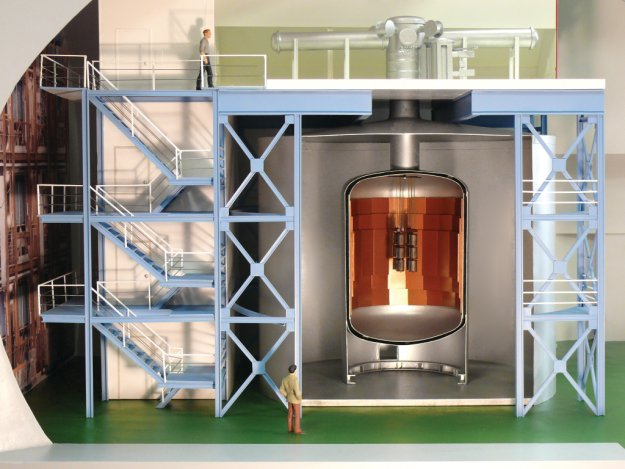
\includegraphics[width=\textwidth]{img/GERDAmodel}};
		\node(a) at (1.9,-1.5) [rectangle,draw,fill] {LAr};
		\node(b) at (4,1.6) [rectangle,draw,fill] {\ce{^76Ge} \textsc{detectors}};
		\draw[thick,red,->] (b.south) .. controls +(0,0) and +(1,0) .. (1.9,-0.4);
		\node(c) at (-1.5,1.6) [rectangle,draw,fill] {\textsc{water tank}};
		\draw[thick,red,->] (c.south) .. controls +(0,0) and +(-1,0) .. (0,-1);
		\node(d) at (0,3) [rectangle,draw,fill] {\textsc{copper shielding}};
		\draw[thick,red,->] (d.south) .. controls +(0,0) and +(-1,0) .. (1,0);
	\end{tikzpicture}
	\caption{Artists view (Ge array not to scale) of the Gerda experiment.}
	\label{artistview}
\end{figure}
\begin{figure}
	\centering
	\resizebox{\textwidth}{!}{
		\includegraphics[height=15cm]{img/strings}%
		\hspace{0.1cm}%
		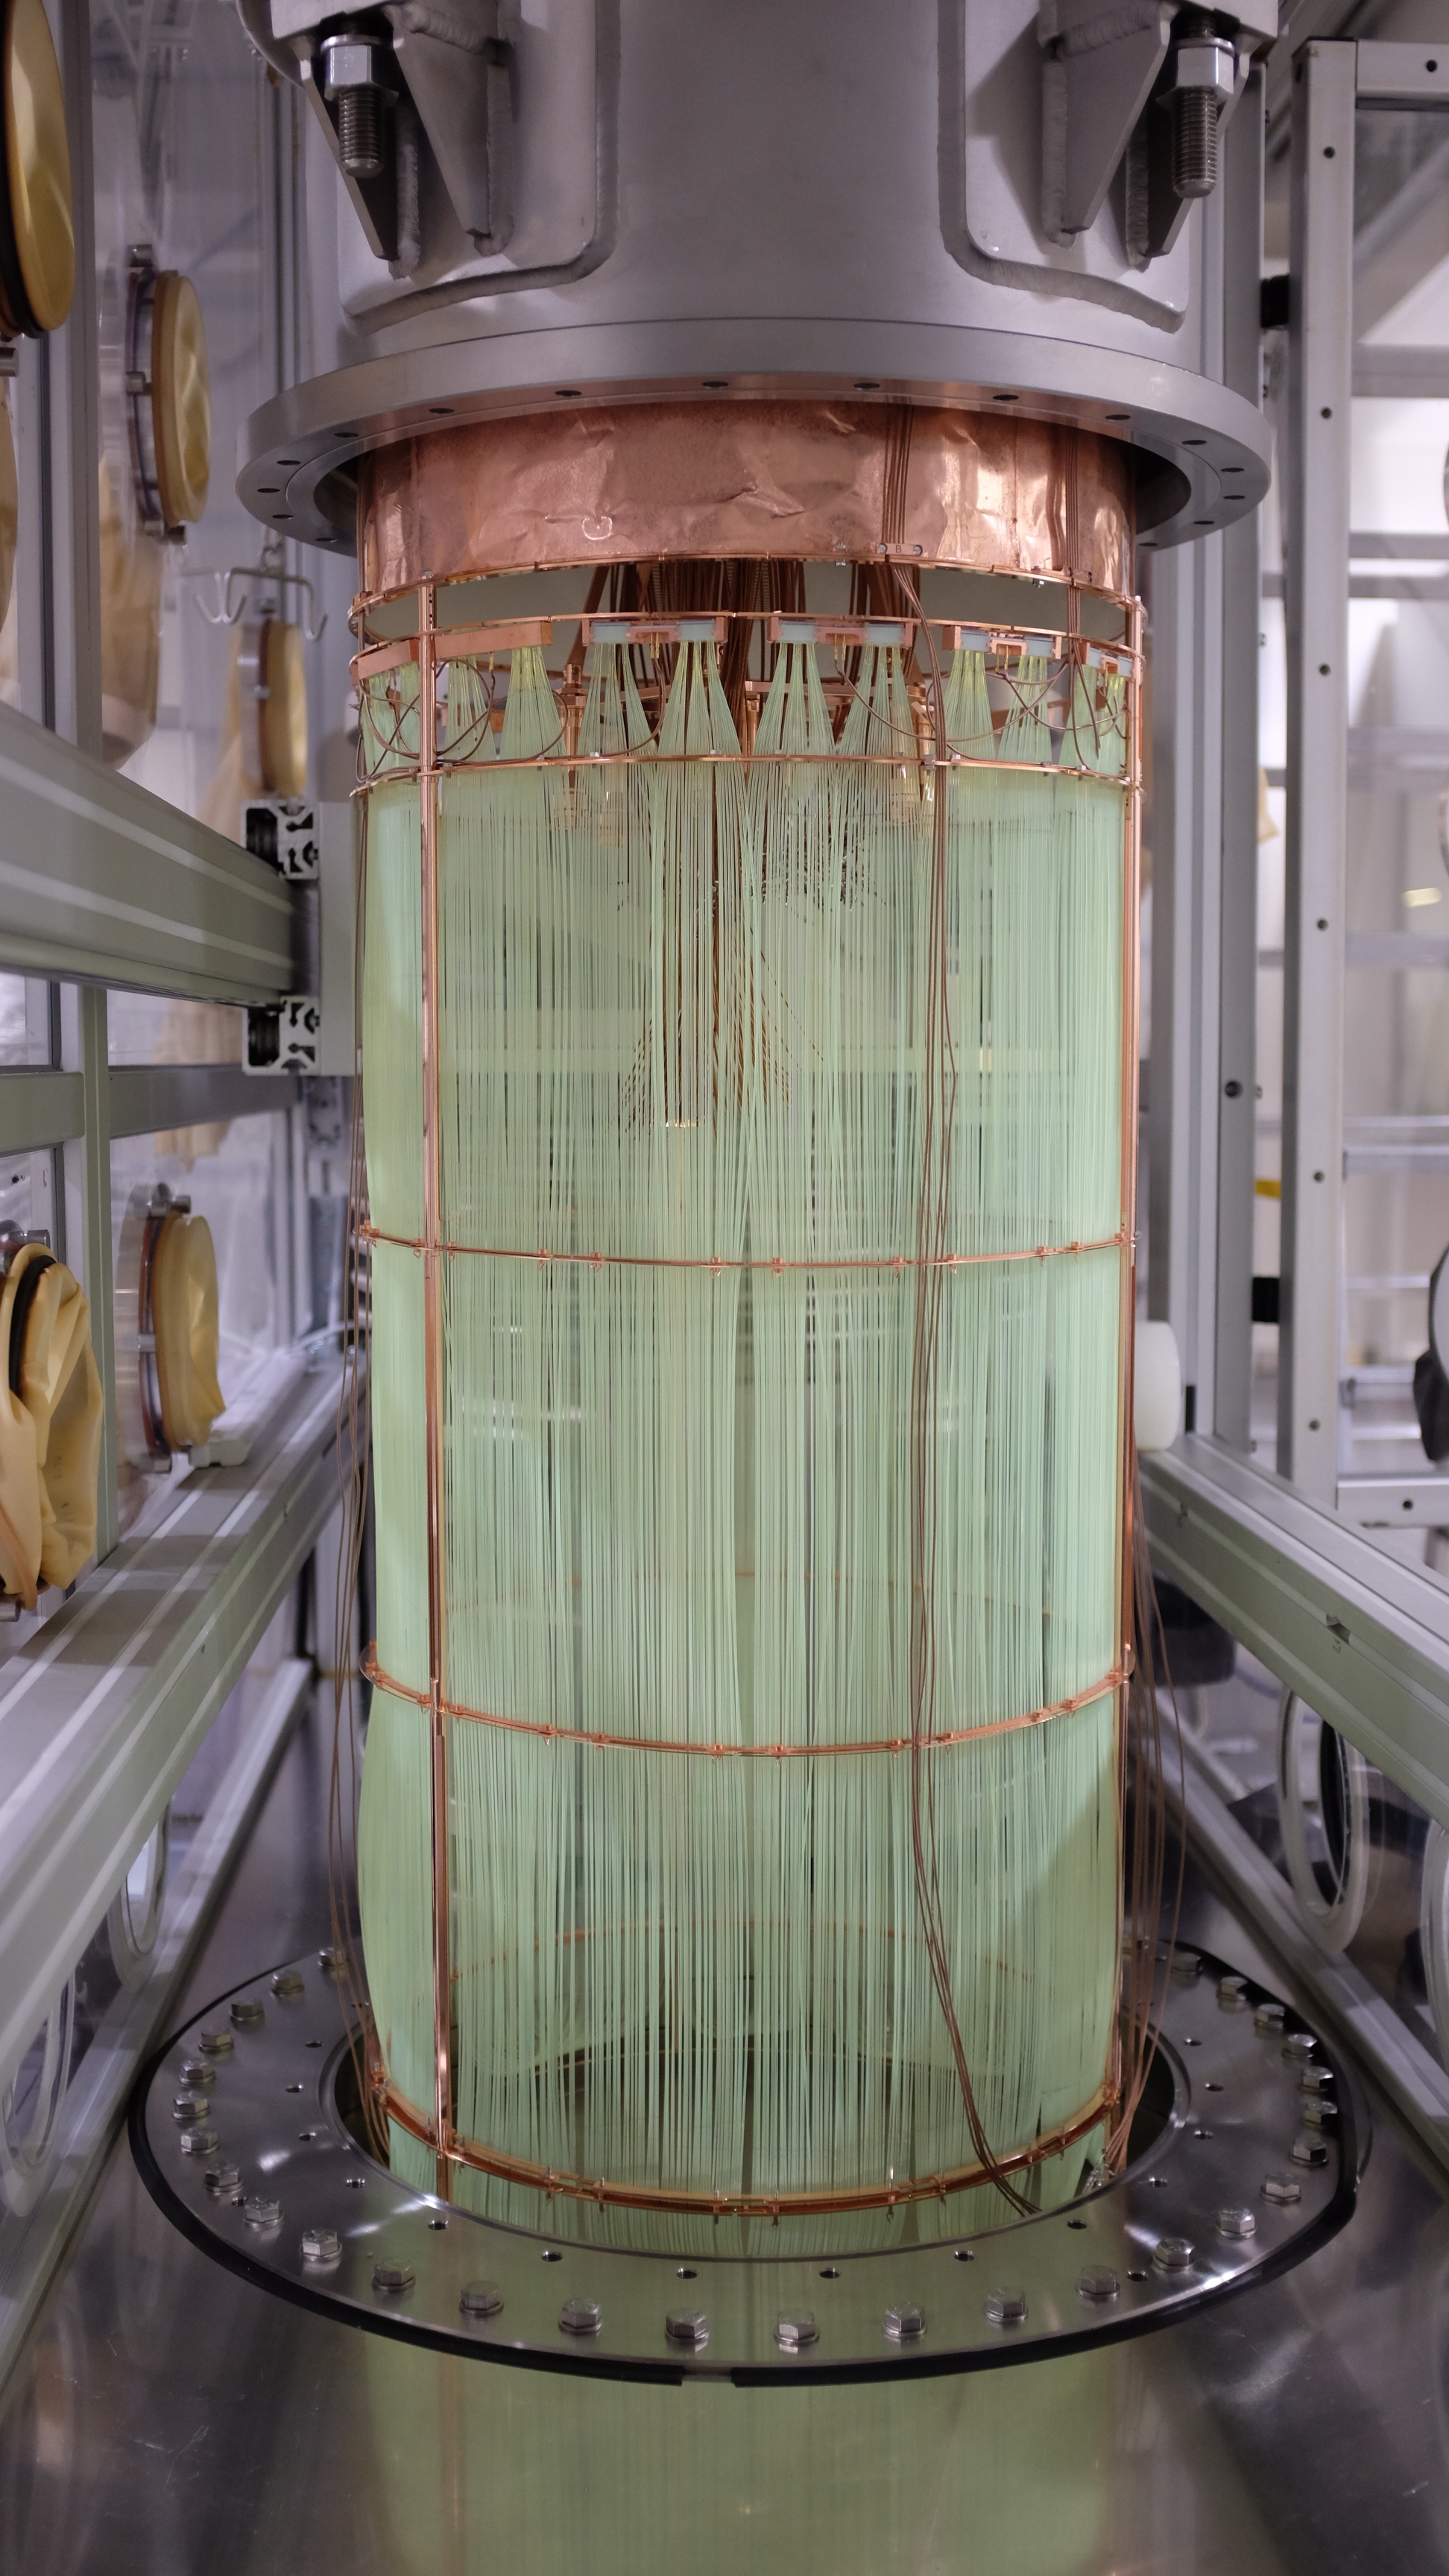
\includegraphics[height=15cm]{img/fibers}%
	}%
	\caption{On the left: some detector strings. On the right: the fiber shroud being submerged in LAr?}
\end{figure}
\begin{figure}
	\centering
	\makebox[\textwidth]{\includegraphics[width=\textwidth]{img/water_tank}}
	\caption{Inside the water tank after the installation of the muon veto system.}
\end{figure}

Fig.~\ref{artistview} shows a model of the realized design: the core of the experiment is an array of germanium diodes suspended in strings into a cryostat filled with LAr. The LAr serves both as cooling medium and shield. The cryostat is a steel vessel with a copper lining used primarily to reduce the gamma radiation from the steel vessel. The cryostat is placed in a large water tank, that fulfills the functions of shielding the inner volumes from radiation sources within the hall, such as neutrons, as well as providing a sensitive medium for a muon veto system. The detectors are lowered into the LAr volume using a lock system located in a clean room on top of the water tank. A further muon veto system is placed on top of the clean room in order to shield the neck region of the cryostat. A detailed description of the experimental setup for phase \textsc{i} is provided in \cite{gerdadescription}.

Phase \textsc{ii} came with some upgrades to improve the background rejection performance. The volume directly surrounding the detector array was instrumented with photo multipliers to detect the scintillation light emitted if energy is deposited inside LAr. This allows to identify background events resulting from Compton scattered photons with partial energy deposit in the detectors and partial energy deposit inside the LAr. Additionally, a curtain made from light guide fibers with tetraphenyl butadiene (TPB) deposited on their surface will surround the detector array. Photons reaching the light guides are wavelength shifted and guided to the end of the fibers, where they can be detected by silicon photomultipliers (SiPMs) optically coupled to the fibers. In principle the new components should improve the identification of background events. In Phase \textsc{i} the individual detector strings were surrounded by a copper shroud, minimizing the LAr volume from which \ce{^{42}K} ions can be collected on the detector surfaces. Additionally the shrouds were set to ground potential to minimize drift towards the detectors. In order to take maximum advantage of the light instrumentation of the LAr, in Phase \textsc{ii} the copper shroud has been be exchanged by a transparent TPB-coated shroud that allows to minimize the volume from which \ce{^{42}K} ions are collected, while allowing to detected scintillation light also from the volume inside the mini shroud. Last but not least, 30 new BEGe detectors were deployed into the LAr.

\marginnote{\textsc{The germanium detectors}} For Phase \textsc{i} all eight detectors from the former \textsc{HdM} \cite{hdm}and \textsc{Igex} \cite{igex} experiments were refurbished and redeployed, In addition, six detectors made of \ce{^{na}Ge} are available from the GENIUS-TF experiment \cite{genius1, genius2}. For Phase \textsc{ii} new material amounting to 50 kg \ce{^{enr}GeO2} was purchased in order to produce new diodes.

\bibliographystyle{unsrt}
\bibliography{bib-thesis}
\end{document}
